\documentclass{beamer}

\usetheme[hideothersubsections,numbers,sidebarshades]{Uppsala}
%\title[Evaluation of a new aligner]{Evaluation of a New Aligner for Ultra-Short Ancient DNA}
\title[Making the Most of Ancient DNA]{Making the Most of Ancient DNA}
\author[Homa Amini]{Homa Amini }
\date[Oct 2016]{October 27, 2016 \\
\vskip .45cm
%\includegraphics[height=2.cm,width=2.5cm]}}
\includegraphics[height=1.75cm,width=1.75cm]{UUL.jpg}}
%\includegraphics[height=2cm,width=2cm]{UU_logo.pdf}}
\institute[MPI-EVA]{
%\includegraphics[height=1cm,width=2cm]{mpi.png}
Max-Planck Institute for
Evolutionary Anthropology\\
Leipzig, Germany }

\usepackage[absolute,overlay]{textpos}

%\usepackage{floatrow}
\usepackage[english]{babel}
\usepackage[utf8x]{inputenc}
\usepackage{graphicx}
\usepackage{subfig}
\usepackage[final]{pdfpages}
\usepackage{float}
\usepackage{caption}
\usepackage[super,negative]{nth}
\usepackage{courier}

\usepackage[export]{adjustbox}
\usepackage{textpos}
\usepackage{multicol}
\usepackage{multirow}
\usepackage{tikz-qtree}
\usepackage{tikz}
\usepackage{multicol}
\usepackage{multirow} 
\usepackage{color}


\definecolor{candyapplered}{rgb}{1.0, 0.03, 0.0}

\usetikzlibrary{tikzmark}
\usetikzlibrary{arrows.meta}

\usetikzlibrary{arrows, automata}

\captionsetup[subfigure]{labelformat=empty} % to remove captions on subfloat figures

%\newcommand{\source}[1]{\begin{textblock*}{4cm}(8.7cm,8.6cm)
\newcommand{\source}[1]{\begin{textblock*}{4cm}(8.7cm,8.6cm)
    \begin{beamercolorbox}[ht=0.5cm,right]{framesource}
        \usebeamerfont{framesource}\usebeamercolor[fg]{framesource} Source: {#1}
    \end{beamercolorbox}
\end{textblock*}}


\begin{document}

\begin{frame}[plain]
  \titlepage
\end{frame}


%%%%%%%%%%%%%%%%%%%%%%%%%%%%%%%%%%%%%%%%%%%%%%%%%%%%%%%%%%%%%%%%%%%%%%%%%%

\section{Specification and Properties of the Data}

\begin{frame}{Why Study Ancient DNA}


\begin{figure}
	
	\subfloat[]{\includegraphics[width=2.1in]{pics/Nean.jpg}}
	\subfloat[]{\includegraphics[width=.689in]{pics/skullss.jpg}} \hspace*{2cm}



	\source{www.sciencemag.org}
 
\end{figure}


\end{frame}







%%%%%%%%%%%%%%%%%%%%%%%%%%%%%%%%%%%%%%%%%%%%%%%%%%%%%%%%%%%%%%%%%%%%%%%%%%

\begin{frame}{What is a DNA Sequence}
\begin{tabular}{cl}  
         \begin{tabular}{l}
          \parbox{0.5\linewidth}{%  change the parbox width as appropiate
           
\begin{itemize}
    
	\item Let $X$ be a sequence of $\lambda$ random variables.  
	$ X =  \left\{ X_{1}, X_{2}, ... , X_{\lambda} \right\} $ which 
	takes the values \hspace{45pt}
	from the alphabet $\left\{A, C, G, T \right\}$.
\end{itemize}
     }
           \end{tabular}
           & \begin{tabular}{l}
            
                  \includegraphics[height=3.3cm, width=4.1cm]{pics/dna-structure.png} 
			 \end{tabular}  \\
           
\end{tabular}
% \source{medivizor.com} 

	\begin{itemize}
  		\item e.g. ACGGCTAAGTCAGATACAGCTCGCA
  	\end{itemize}	
\begin{figure}
	\includegraphics[width=4.5cm]{pics/seq2.png}


	 \source{medivizor.com\\ 
	http://www.genomenewsnetwork.org}
 
\end{figure}\end{frame}
%%%%%%%%%%%%%%%%%%%%%%%%%%%%%%%%%%%%%%%%%%%%%%%%%%%%%%%%%%%%%%%%%%%%%%%%%%


\begin{frame}[shrink=20]
\frametitle{What is Ancient DNA}

\begin{figure}
	
	\subfloat[]{\includegraphics[width=2.1in]{pics/bone.jpg}}
	\subfloat[]{\includegraphics[width=.8381in]{pics/fingertip.jpg}} \hspace*{2cm}
	

	\source{Meyer M,et al. Science 2012 \& \\
	http://www.ourdailyread.com/2014/02/}
 
\end{figure}


  Let lowercase $x =\left\{ x_{1}, x_{2}, ... , x_{\lambda}\right\}$ 
  represent a specific DNA sequence.
  \begin{itemize}
  		\item e.g. ATTGTTACAGATATT
  	\end{itemize}
 \vskip .5cm 
 \textbf{Characteristics}


\begin{itemize}

	\item Hard to retrieve. 
	\item Short molecule $\leq$ 50 bp.
	\item \emph{Post-Mortem} damage: deamination (substitutions of C$\to$T).
	\item Microbial contamination.
\end{itemize}

\end{frame}

%%%%%%%%%%%%%%%%%%%%%%%%%%%%%%%%%%%%%%%%%%%%%%%%%%%%%%%%%%%%%%%%%%

\begin{frame}{\emph{Post-Mortem} Deamination Damage}

\begin{figure}
\centering
	\includegraphics[width=10cm]{pics/substitution_pattern.png}

	\source{http://mitosuite.com/example/results.html}
\end{figure}

A high nucleotide misincorporation rate of thymine(T) in place of
cytosine(C) near the ends of ancient DNA reads.

\end{frame}


%%%%%%%%%%%%%%%%%%%%%%%%%%%%%%%%%%%%%%%%%%%%%%%%%%%%%%%%%%%%%%%%%%



%%%%%%%%%%%%%%%%%%%%%%%%%%%%%%%%%%%%%%%%%%%%%%%%%%%%%%%%%%%%%%%%%



\begin{frame}{Sequencer}
\begin{itemize}
	\item A sequencer is a machine used to determine the order of DNA bases.
\end{itemize}
\begin{figure}
%\centering

%	\subfloat[]{\includegraphics[width=1.7in]{pics/seq2.png}}
	\subfloat[]{\includegraphics[width=6.5cm]{pics/illumina.jpg}} %\hspace*{2cm}


	\source{http://www.illumina.com }
%	http://www.genomenewsnetwork.org}
 
\end{figure}


\end{frame}

%%%%%%%%%%%%%%%%%%%%%%%%%%%%%%%%%%%%%%%%%%%%%%%%%%%%%%%%%%%%%%%%%

\section{Common Approaches to String Alignments}
\begin{frame}{DNA Similarity}

\begin{itemize}

	%\item DNA sequences may have changed from an evolutionary origin 
	\item DNA sequences may have changed from a common ancestor 
	through various reasons:\\
	
	\begin{itemize}
		\item Change of a letter\\
			
				 \hspace{85pt} \textbf{\texttt{AC\textcolor{candyapplered}{G}CTATGCA}} \\
				\hspace{85pt} \textbf{\texttt{AC\textcolor{candyapplered}{C}CTATGCA}}
			
		\item Insertion of a letter\\
			
				  \hspace{85pt} \textbf{\texttt{ACGCTATGC\textcolor{candyapplered}{-}A}} \\
				 \hspace{85pt} \textbf{\texttt{ACGCTATGC\textcolor{candyapplered}TA}}
			
		\item Deletion of a letter\\
			
				 \hspace{85pt} \textbf{\texttt{ACGCT\textcolor{candyapplered}{A}TGCA}} \\
				 \hspace{85pt} \textbf{\texttt{\texttt{ACGCT\textcolor{candyapplered}{-}TGCA}}}
			
	\end{itemize}
	\vskip .25cm
	\item A few mutations make sequences different, but still
	“similar” and we are looking for these similarities.
\end{itemize}

\end{frame}
%%%%%%%%%%%%%%%%%%%%%%%%%%%%%%%%%%%%%%%%%%%%%%%%%%%%%%%%%%%%%%%%%

\begin{frame}[shrink=1]
\frametitle{DNA Sequence Alignment}

\begin{itemize}
	
	\item Alignment to the reference genome to identify \\
	the molecules we are interested in. 

	\item Approximate pattern matching.
	
	\item e.g.\\
			\hspace{45pt}	$S_{1}:$\hspace{25pt} \textbf{\texttt{ACGCTATAGCA}}\\
%\vskip .5cm			
			\hspace{45pt}	$S_{2}:$\hspace{25pt} \textbf{\texttt{CGATGAC}} 
\vskip .5cm 
		
		A plausible alignment of $S_{1}$ and $S_{2}$:	
\vskip .5cm 
		\hspace{45pt} $S_{1}:$\hspace{25pt} \textbf{\texttt{ACGCTATAGCA\textcolor{candyapplered}{-}}}\\
		\hspace{45pt} $S_{2}:$\hspace{25pt} \textbf{\texttt{\textbf{\textcolor{candyapplered}{-}}CG\textbf{\textcolor{candyapplered}{--}}AT\textbf{\textcolor{candyapplered}{-}}G\textcolor{candyapplered}{-}}AC} \\
\end{itemize}

\end{frame}

%%%%%%%%%%%%%%%%%%%%%%%%%%%%%%%%%%%%%%%%%%%%%%%%%%%%%%%%%%%%%%%%%%%


%\begin{frame}{Three Key Questions }

%\begin{itemize}
%	\item  Q1: What do we want to align?
%	\item  Q2: How do we "score" an alignment?.
%	\item  Q3: How to find the "optimal" alignment?.
%\end{itemize}

%\end{frame}

%%%%%%%%%%%%%%%%%%%%%%%%%%%%%%%%%%%%%%%%%%%%%%%%%%%%%%%%%%%%%%%%%%%%

%\begin{frame}{What Sort of Alignment? }
\begin{frame}[shrink=30]

\frametitle {What Sort of Alignment? }

\vskip .5cm

\begin{itemize}
\item \textbf{Global alignment:} \\
\vskip .25cm

$S_{1}:$\hspace{10pt}\textcolor{red}{ACCGT}CGCTACTGCTGT..............CAG\textcolor{candyapplered}{ATCGC}TCATCGCATA\textcolor{candyapplered}{CTGTCT}\\
$S_{2}:$\hspace{10pt}\textcolor{candyapplered}{ACCGT}GTA ......... CAGATCGCTCATC\textcolor{candyapplered}{ATCGC}AGTCGATAGC\textcolor{candyapplered}{CTGTCT}\\

\vskip 1cm

\item \textbf{Local alignment:}
\vskip .25cm

$S_{1}:$\hspace{10pt} ACCGTCGCTACTGCTGTC\textcolor{candyapplered}{AGATCGCTCA}GTTCGATCTG\\
$S_{2}:$\hspace{77pt}GTCTGTCAG\textcolor{candyapplered}{AGATCGCTCA}TCGCATACTGTCTCGTCC\\

\vskip 1cm

\item \textbf{Semi-Global alignment:}
\vskip .25cm 

$S_{1}:$\hspace{10pt} ACCGTCGCTACTGCTGTC\textcolor{candyapplered}{AGATCGCTCA}GTTCGCTGTCAAGTCACT\\
$S_{2}:$\hspace{77pt}\hspace{65pt}\textcolor{candyapplered}{AGATCGCTCA}\\

\end{itemize}
\end{frame}



%%%%%%%%%%%%%%%%%%%%%%%%%%%%%%%%%%%%%%%%%%%%%%%%%%%%%%%%%%%%%%%%%%%%
\begin{frame}[shrink=20]
\frametitle {Scoring an Alignment }

%\begin{frame}{Scoring an Alignment }

\begin{itemize}

	\item The alignment score is the sum of all the scores of paired aligned
		  characters plus the gap scores.
	
	\item e.g. substitution matrix %for DNA sequence alignment:
		%$$HE\_LLO $$
 		%$$H\_ALLO $$
 		
 %		\resizebox{\textwidth}{12}{
		\begin{table}[H]
		% \centering
		 %\begin{adjustbox}{max width=\textwidth}
		  
		  \begin{tabular}{  c| r  r r  r }
    
			   $S(S_{1i},S_{2j})$  & A & C &  G & T \\ \hline
	          A &  1  & -1 & -1 & -1 \\
              C & -1  &  1 & -1 & -1 \\ 
       		  G & -1  & -1 &  1 & -1 \\ 
       		  T & -1  & -1 & -1 &  1 \\
	     \end{tabular}
		%\caption{comparation between modern DNA and ancient DNA}
		%\label{alignment-exp}
		%\end{adjustbox}
	  \end{table}
%}
 	
 	If g = $-1$% the score of following alignment is:
 
		\begin{center}
			\begin{tabular}{c *{12}cccc}
				
				%	\hline
        		$S_{1}:$\hspace{8pt} & & C & C & G & A & \textbf{\textcolor{candyapplered}{-}} & T & A  \\
				%\hline
		    	$S_{2}:$\hspace{8pt} & & T & C & G &  \textbf{\textcolor{candyapplered}{- }} & C  &  T & A \\
    	                                 
			\end{tabular}
		\end{center} 
	\vskip.5cm
we score it by:\\
	$$ 	S(C,T) + S(C,C) + S(G,G) + 2g + S(T,T) +S(A,A) $$ 
	$$-1 + 1 + 1 - 1 - 1 + 1 + 1 = 1$$
 		
\end{itemize}
	
\end{frame}

%%%%%%%%%%%%%%%%%%%%%%%%%%%%%%%%%%%%%%%%%%%%%%%%%%%%%%%%%%%%%%%%%%%%

\begin{frame}{ How to Find the Optimal Alignment? }

\begin{itemize}
	\item Simple approach: Compute and score all possible
	alignments.
	\vskip 0.35cm
	There are:
		$$ \binom{2n}{n} = \frac{(2n)!}{(n!)^2} \simeq \frac{2^{2n}}{\sqrt{2\pi n}} $$
		\vskip 0.2cm
		global alignments.
	\begin{itemize}	 
		\item Time complexity $\mathcal{O}(2^{2n})$.
	\end{itemize}	
	\vskip 0.25cm		
	\item Dynamic programming
		\begin{itemize}
			\item Calculate the best alignment of all prefixes of the sequences instead of best alignment of the two sequences.
			%\item reuse the scores already considered.
			\item  Time complexity $\mathcal{O}(n^{2})$.
		\end{itemize}
\end{itemize}

\end{frame}

%%%%%%%%%%%%%%%%%%%%%%%%%%%%%%%%%%%%%%%%%%%%%%%%%%%%%%%%%%%%%%%%%%%%

%%%%%%%%%%%%%%%%%%%%%%%%%%%%%%%%%%%%%%%%%%%%%%%%%%%%%%%%%%%%%%%%%%%%
\begin{frame}{ Overview of BWA Aligner}
	\begin{itemize}
		\item Based on FM-index.
		(Burrows-Wheeler Transform plus auxiliary data structures)
		which enables fast matching. 
		  %    It can be used to simulate a suffix tree, it allows quick access 
		   %   (pattern match in $\mathcal{O}(|p|)$, location in $\mathcal{O}(log n)$, it is reasonably compact.
     	\item Fast and moderate memory footprint ($<$4GB).
		\item Backtracking algorithm with heuristics.
		%\item Seed heuristics: set a limit on the number of allowed mismatches in
		%the few tens of bases on a read sequence.
		\item Seed heuristic.
		\item Does not take deamination into consideration.
	\end{itemize}
\end{frame}

%%%%%%%%%%%%%%%%%%%%%%%%%%%%%%%%%%%%%%%%%%%%%%%%%%%%%%%%%%%%%%%%%%%%
\begin{frame}{ Why is a New Aligner Needed?}


	\begin{itemize}
				
		\item Alignment 1:\\

		 \hspace{55pt}\textbf{\texttt{A\textcolor{candyapplered}{CCC}ACTCTACCTCATCGA\textcolor{candyapplered}{CC}}}\\ 
		 \hspace{55pt}\textbf{\texttt{A\textcolor{candyapplered}{TTT}ACTCTACCTCATCGA\textcolor{candyapplered}{TT}}}\\
		
			\vskip.5cm
			
		\item Alignment 2:\\
			\vskip.5cm
			
			\hspace{55pt}\textbf{\texttt{\textcolor{candyapplered}{A}CCC\textcolor{candyapplered}{A}CT\textcolor{candyapplered}{C}TACC\textcolor{candyapplered}{T}C\textcolor{candyapplered}{A}TCGACC}}\\
			\hspace{55pt}\textbf{\texttt{\textcolor{candyapplered}{C}CCC\textcolor{candyapplered}{T}GT\textcolor{candyapplered}{T}TACC\textcolor{candyapplered}{A}C\textcolor{candyapplered}{C}TCGACC}}
			%\vskip.5cm

		
	\end{itemize}

\end{frame}

%%%%%%%%%%%%%%%%%%%%%%%%%%%%%%%%%%%%%%%%%%%%%%%%%%%%%%%%%%%%%%%%%%%%%
%\section{Evaluation of the New Approach}
\begin{frame}{ R-Candy: New Aligner for Ancient DNA }

\begin{itemize}

	\item Aligns ultra-short reads of length $\leq$ 35bp.
	\item Copes with high levels of specific damage expected in ancient DNA. 		  
	
\end{itemize}

\begin{figure}
%\centering
\subfloat[]{\includegraphics[width=1.20 in]{pics/candyZ.png}}\hspace*{0.15 cm}
\subfloat[]{\includegraphics[width=.65 in]{pics/noteq.jpg}} \hspace*{0.05 cm}
\subfloat[]{\includegraphics[width=2 in]{pics/irf.png}} %\hspace*{2cm}
 
\source{http://www.5ideas.in} 
%\label{fig:EcUND} 
\end{figure}

\end{frame}

%%%%%%%%%%%%%%%%%%%%%%%%%%%%%%%%%%%%%%%%%%%%%%%%%%%%%%%%%%%%%%%%%%%%

\begin{frame}{Overview of R-Candy's Algorithm}
	\begin{itemize}
		\item Based on FM-index (Burrows-Wheeler Transform plus auxiliary 
		      data structures) which enables fast matching.
		\item Backtracking on FM-index. 
		\item Implements a model for damage expected on ancient DNA.
		\item Tailored for short reads of ancient DNA.
	\end{itemize}
\end{frame}

%%%%%%%%%%%%%%%%%%%%%%%%%%%%%%%%%%%%%%%%%%%%%%%%%%%%%%%%%%%%%%%%%%%%


\section{Evaluation of the New Approach}
\begin{frame}{Test Data }
	\begin{itemize}
		\item To compare sensitivity of R-Candy to BWA aligner.
			\begin{itemize}
				\item Simulated modern and ancient DNA reads originated from a simulated genome.
			\end{itemize}	
		\item To roll out possible artifacts of genome simulation.
			\begin{itemize}
				\item Simulated modern and ancient DNA reads originated from a real genome.
			\end{itemize}
		\item To evaluate the rate of false positive alignments.
			\begin{itemize}
				\item Simulated random reads as stands for exogenous DNA.
			\end{itemize}
	\end{itemize}
\end{frame}
%%%%%%%%%%%%%%%%%%%%%%%%%%%%%%%%%%%%%%%%%%%%%%%%%%%%%%%%%%%%%%%%%%%%%	


%\begin{frame}{\nth{1} Order Markov Chain}

\begin{frame}{Genome Simulation}
\begin{figure}[H]
 \begin{center}
	  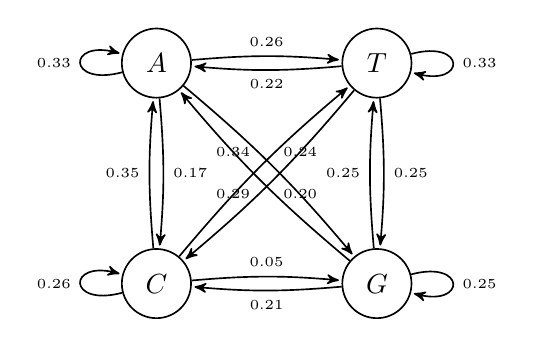
\begin{tikzpicture}[->,>=stealth',shorten >=1pt,auto,node distance=2.8cm,
                    semithick,bend angle=5]
   \tikzstyle{every state}=[fill=white,draw=black,text=black]

   \node[state]         (A)              {$A$};
   \node[state]         (T) [right of=A] {$T$};
   \node[state]         (C) [below of=A] {$C$};
   \node[state]         (G) [below of=T] {$G$};
  
   \path (A) edge [bend left]  node {\tiny 0.26} (T)
  			edge [loop left] node {\tiny 0.33} (A)
            edge [bend left]  node {\tiny 0.17} (C)
            edge [bend left]  node {\tiny 0.24} (G)
        (T) edge [loop right] node {\tiny 0.33} (T)
            edge [bend left]  node {\tiny 0.22} (A)
            edge [bend left]  node {\tiny 0.20} (C)
            edge [bend left]  node {\tiny 0.25} (G)
        (C) edge [bend left]  node {\tiny 0.34} (T)
            edge [loop left] node {\tiny 0.26} (C)
            edge [bend left]  node {\tiny 0.05} (G)
            edge [bend left]  node {\tiny 0.35} (A)
        (G) edge [loop right] node {\tiny 0.25} (G)
       	    edge [bend left]  node {\tiny 0.21} (C)
        	edge [bend left]  node {\tiny 0.29} (A)
            edge [bend left]  node {\tiny 0.25} (T);
  \end{tikzpicture}
  
  Trained \nth{1} order Markov chain based on the human reference genome.
 
 \end{center}
\end{figure}


\end{frame}

%%%%%%%%%%%%%%%%%%%%%%%%%%%%%%%%%%%%%%%%%%%%%%%%%%%%%%%%%%%%%%%%%%%%%%

\begin{frame}[shrink=1.75]
\frametitle {\nth{1} Order Markov Chain }
	

\begin{figure}[H]
 \begin{center}
 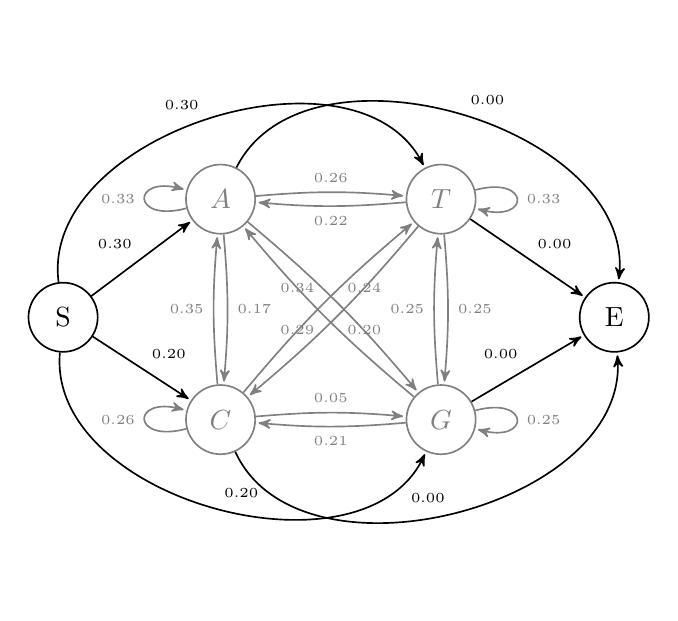
\begin{tikzpicture}[->,>=stealth',shorten >=1pt,auto,node distance=2.8cm,
                    semithick,bend angle=5]
  \tikzstyle{every state}=[fill=white,draw=gray,text=gray]

  \node[state]         (A)              {$A$};
  \node[state]         (T) [right of=A] {$T$};
  \node[state]         (C) [below of=A] {$C$};
  \node[state]         (G) [below of=T] {$G$};
  \node[state]         (S) [draw=black, text= black]at (-2,-1.5) {S};
  \node[state]         (E) [draw=black, text = black]at (5 ,-1.5) {E};
  
  \path (A) edge [gray, bend left]  node {\tiny 0.26} (T)
  			edge [gray, loop left] node {\tiny 0.33} (A)
            edge [gray, bend left]  node {\tiny 0.17} (C)
            edge [gray, bend left]  node {\tiny 0.24} (G)
            edge [bend left=80]  node {\tiny 0.00} (E)
        (T) edge [gray, loop right] node {\tiny 0.33} (T)
            edge [gray, bend left]  node {\tiny 0.22} (A)
            edge [gray, bend left]  node {\tiny 0.20} (C)
            edge [gray, bend left]  node {\tiny 0.25} (G)
            edge   			  node {\tiny 0.00} (E)
        (C) edge [gray, bend left]  node {\tiny 0.34} (T)
            edge [gray, loop left] node {\tiny 0.26} (C)
            edge [gray, bend left]  node {\tiny 0.05} (G)
            edge [gray, bend left]  node {\tiny 0.35} (A)
            edge [bend right=80]  node {\tiny 0.00} (E)
        (G) edge [gray, loop right] node {\tiny 0.25} (G)
       	    edge [gray, bend left]  node {\tiny 0.21} (C)
        	edge [gray, bend left]  node {\tiny 0.29} (A)
            edge [gray, bend left]  node {\tiny 0.25} (T)
            edge   			  node {\tiny 0.00} (E)
        (S) edge   			  node {\tiny 0.30} (A)
       	    edge   			  node {\tiny 0.20} (C)
        	edge [bend right=80]  node {\tiny 0.20} (G)
            edge [bend left=80]  node {\tiny 0.30} (T)
       
            ;
;
 \end{tikzpicture}

Trained \nth{1} Order Markov-Chain based on the human reference genome with start and end states
 \end{center}
\end{figure}
% Trained \nth{1} Order Markov-Chain based on the human reference genome with start and end states

\end{frame}


%%%%%%%%%%%%%%%%%%%%%%%%%%%%%%%%%%%%%%%%%%%%%%%%%%%%%%%%%%%%%%%%%%%%%%

\begin{frame}{Read Simulation (Cont.) }
\begin{figure}[H]
\centering
\includegraphics[width=10cm]{pics/readsampling2.png}
%\caption{Number of bases in each cycle as a function of having certain quality}
\label{hist}
\end{figure}
\end{frame}


%%%%%%%%%%%%%%%%%%%%%%%%%%%%%%%%%%%%%%%%%%%%%%%%%%%%%%%%%%%%%%%%%%%%%%%

%\begin{frame}[shrink=30]
%\frametitle{Read Simulation (Cont.)}
\begin{frame}{Read Simulation (Cont.)}
\begin{itemize}
		\item \textbf{Divergence}: different divergence rates are simulated by a given number of mismatches per read. 
		%\item \textbf damage}: taking into account being in overhangs with different damage rate.
		\item \textbf{Deamination damage}: based on 
			  deamination parameters (overhang ($\sigma$) and double stranded ($\delta$) deamination 
			  rates plus the probability of being in overhangs) provided by users.
		\vskip .25cm	  
		\begin{figure}[H]
		\centering
			%\includegraphics[width=5.5cm]{pics/CalOverhang.pdf}
			%\includegraphics[width=2.5cm]{pics/OverhangLength.png}
			
			\subfloat[]{\includegraphics[width=4.5cm]{pics/CalOverhang.pdf}}\hspace*{.009cm}
			\subfloat[]{\includegraphics[width=4cm]{pics/OverhangLength.png}} \hspace*{.5cm}



		\end{figure}
		
\end{itemize}
\end{frame}
%%%%%%%%%%%%%%%%%%%%%%%%%%%%%%%%%%%%%%%%%%%%%%%%%%%%%%%%%%%%%%%%%%%%%%%

%\begin{frame}[shrink=.50]
%\frametitle{Read Simulation (Cont.)}
\begin{frame}{Read Simulation (Cont.)}
\begin{itemize}
\item \textbf{Sequencing error}: specific types of errors introduced by the sequencing 
			   machine based on the distribution of quality scores on an actual sequencing run.\\
		\begin{figure}[H]
			\centering
			\includegraphics[width=7cm]{pics/3D.png}
			\label{hist}
		\end{figure}
%\footnotesize	Number of bases in each cycle as a function of having certain quality.	
\end{itemize}
\end{frame}
%%%%%%%%%%%%%%%%%%%%%%%%%%%%%%%%%%%%%%%%%%%%%%%%%%%%%%%%%%%%%%%%%%%%%%%
\begin{frame}[shrink=15]
\frametitle{Read Simulation (Cont.)}
%\begin{frame}{Read Simulation (Cont.)}
\vskip 2.5cm
\begin{table}[ht]
\centering
\begin{adjustbox}{max width=\textwidth}
\begin{tabular}{|p{3cm}|c|c|c|}\cline{2-4}


\multicolumn{1}{c|}{} & \textbf{Divergence} & \textbf{Deamination} & \textbf{Sequencing } \\
\multicolumn{1}{c|}{} &  & \textbf{Damage }& \textbf{ Error} \\
\hline 
\textbf{Modern DNA} & \checkmark & & \checkmark  \\\hline

\textbf{Ancient DNA} & \checkmark &\checkmark  & \checkmark  \\\hline

\textbf{Exogenous DNA} &  & \checkmark &  \checkmark  \\\hline

\end{tabular}
\end{adjustbox}
%\caption{Evaluation test scenarios}
\label{test-scenarios}
\end{table}

\end{frame}

%%%%%%%%%%%%%%%%%%%%%%%%%%%%%%%%%%%%%%%%%%%%%%%%%%%%%%%%%%%%%%%%%%%%%%
\begin{frame}{Evaluation Criteria}
\begin{tabular}{cl}  
         \begin{tabular}{l}
          \parbox{0.45\linewidth}{%  change the parbox width as appropiate
           \begin{itemize}
			\item  \textbf{Mapping accuracy}:
		{	\scriptsize		
			
			 \[ \textbf{Sensitivity} (TPR) = \dfrac{\# TP }{\# TP + \# FN} \]
 			 \[ \textbf{Specificity} (TNR) = \dfrac{\# TN }{\# TN + \# FP} \]
 		}
 			\end{itemize}
 			}
           \end{tabular}
           & \begin{tabular}{l}
            
            	%\begin{figure}
	              \includegraphics[height=3.3cm, width=4.3cm]{pics/TPFN.png} 
				%   \source{alazycowboy.com} 
    			%\end{figure}
           \end{tabular}  \\
           
\end{tabular}
 \source{alazycowboy.com} 

\begin{itemize}


	\item \textbf{Throughput}: the number of mapped reads per second. 
	\vskip .5cm
	
	\item \textbf{Memory footprint}: required memory for indexing, processing and storing.

\end{itemize}
\end{frame}
%%%%%%%%%%%%%%%%%%%%%%%%%%%%%%%%%%%%%%%%%%%%%%%%%%%%%%%%%%%%%%%%%%%%%%%
%%%%%%%%%%%%%%%%%%%%%%%%%%%%%%%%%%%%%%%%%%%%%%%%%%%%%%%%%%%%%%%%%%%%%%%%%%%%%%%%%%%%%%%%%%%%%%%%%%%%%%%
\begin{frame}{Evaluation Scenarios}
\begin{table}[ht]
\centering
\begin{adjustbox}{max width=\textwidth}
\begin{tabular}{|c|c|c|c|c|c|c|}\cline{2-7}

\multicolumn{1}{c|}{\multirow{2}{*}{}}  &\multicolumn{2}{c|}{\textbf{DNA Reads}} 
&\multicolumn{2}{c|}{\textbf{Aligned To}} 
&\multicolumn{2}{c|}{\textbf{Parameters}}\\\cline{2-7}

\multicolumn{1}{c|}{} & Modern & Ancient & Simulated & Real & Default & Ancient \\
\multicolumn{1}{c|}{} &	& & Genome & Genome & (No Deamination) & \\\hline

 
\textbf{MSD}  & \checkmark &  & \checkmark & & \checkmark & \\\hline

\textbf{MRD} & \checkmark &  & & \checkmark & \checkmark &  \\\hline

\textbf{MSA} & \checkmark  & & \checkmark & &  & \checkmark \\\hline

\textbf{MRA} & \checkmark & & & \checkmark &  & \checkmark  \\\hline

\textbf{ASA} &  & \checkmark  &\checkmark &  & &  \checkmark \\\hline

\textbf{ARA} &  & \checkmark & & \checkmark & &  \checkmark \\\hline


\end{tabular}
\end{adjustbox}
%\caption{Evaluation test scenarios}
\label{test-scenarios}
\end{table}
\scriptsize M = Modern/Fresh DNA\\
A = Ancient DNA/parameters\\
S = Simulated genome\\
R = Real genome\\
D = Default parameters
\end{frame}
%%%%%%%%%%%%%%%%%%%%%%%%%%%%%%%%%%%%%%%%%%%%%%%%%%%%%%%%%%%%%%%%%%%%%%%

\begin{frame}{ROC Curve}

	\begin{figure}[H]
		\centering
		\includegraphics[width=9.5cm]{pics/DS6-25_O.pdf}
%\caption{Number of bases in each cycle as a function of having certain quality}
		
	\end{figure}

\end{frame}
%%%%%%%%%%%%%%%%%%%%%%%%%%%%%%%%%%%%%%%%%%%%%%%%%%%%%%%%%%%%%%%%%%%%%%%%%%




\begin{frame}{\small{Modern DNA Simulated Genome, Default Parameters}}
%\begin{frame}{\footnotesize Evaluation of Modern DNA Reads Aligned to the Simulated Genome 
%by Default Parameters}
	
	\begin{figure}[H]
\centering
\includegraphics[width=7cm]{pics/f_DS3_emp.pdf}
%\caption{Number of bases in each cycle as a function of having certain quality}
%\label{hist}
\end{figure}
\end{frame}

%%%%%%%%%%%%%%%%%%%%%%%%%%%%%%%%%%%%%%%%%%%%%%%%%%%%%%%%%%%%%%%%%%%%%%%%
\begin{frame}{\small{Modern DNA Human Ref Genome, Default Parameters}}
%\begin{frame}{Evaluation of FRD}
	%Alignment of Simulated Modern DNA Reads to the Human Reference Genome with default parameters.
	
	\begin{figure}[H]
		\centering
		\includegraphics[width=7cm]{pics/f_DS6_emp.pdf}
%\caption{Number of bases in each cycle as a function of having certain quality}
		
	\end{figure}

\end{frame}

%%%%%%%%%%%%%%%%%%%%%%%%%%%%%%%%%%%%%%%%%%%%%%%%%%%%%%%%%%%%%%%%%%%%%%%%
\begin{frame}{\small{Modern DNA Simulated Genome, Ancient Parameters}}
%\begin{frame}{Evaluation of FSA}	
	\begin{figure}[H]
		\centering
		\includegraphics[width=7cm]{pics/f_DS8_emp.pdf}
%\caption{Number of bases in each cycle as a function of having certain quality}
		
	\end{figure}

\end{frame}

%%%%%%%%%%%%%%%%%%%%%%%%%%%%%%%%%%%%%%%%%%%%%%%%%%%%%%%%%%%%%%%%%%%%%%%%
\begin{frame}{\small{Modern DNA Human Ref Genome, Ancient Parameters}}
%\begin{frame}{Evaluation of FRA}
	%Alignment of Simulated Modern DNA Reads to a the Human Reference Genome with ancient parameters.}
	\begin{figure}[H]
		\centering
		\includegraphics[width=7cm]{pics/f_DS9_22_20_54_emp.pdf}
%\caption{Number of bases in each cycle as a function of having certain quality}
		
	\end{figure}

\end{frame}
%%%%%%%%%%%%%%%%%%%%%%%%%%%%%%%%%%%%%%%%%%%%%%%%%%%%%%%%%%%%%%%%%%%%%%%
\begin{frame}{\small{Ancient DNA Simulated Genome, Ancient Parameters}}
%\begin{frame}{Evaluation of ASA}	
	%Alignment of Simulated Modern DNA Reads to a Simulated Genome with ancient parameters.
	
	\begin{figure}[H]
		\centering
		\includegraphics[width=7cm]{pics/f_DS1_emp.pdf}
%\caption{Number of bases in each cycle as a function of having certain quality}
		
	\end{figure}

\end{frame}
%%%%%%%%%%%%%%%%%%%%%%%%%%%%%%%%%%%%%%%%%%%%%%%%%%%%%%%%%%%%%%%%%%%%%%
\begin{frame}{\small{Ancient DNA Human Ref Genome, Ancient Parameters}}
%\begin{frame}{Evaluation of ARA}
	\begin{figure}[H]
		\centering
		\includegraphics[width=7cm]{pics/f_DS4_emp.pdf}
%\caption{Number of bases in each cycle as a function of having certain quality}
		
	\end{figure}

\end{frame}


%%%%%%%%%%%%%%%%%%%%%%%%%%%%%%%%%%%%%%%%%%%%%%%%%%%%%%%%%%%%%%%%%%%%%%%
\section{Conclusion \& Future Work}
\begin{frame}{Conclusion}

\begin{tabular}{cl}  
         \begin{tabular}{l}
          \parbox{0.45\linewidth}{%  change the parbox width as appropiate
           \begin{itemize}
			\item R-Candy reduces the minimum read length that can be used for ancient DNA alignment from 35 bp to about 25 bp.
		
 			\end{itemize}
 			}
           \end{tabular}
           & \begin{tabular}{l}
            
            	%\begin{figure}
	              \includegraphics[height=3.3cm, width=4.3cm]{pics/sima_readDis1.png} 
				%   \source{alazycowboy.com} 
    			%\end{figure}
           \end{tabular}  \\
           
\end{tabular}
\source{ Meyer M, et al. Nature 2013}
%Meyer, Matthias, et al. "A mitochondrial genome sequence of a hominin from Sima de los Huesos." Nature } 

\begin{itemize}
	\item Can be used to align both ancient and modern DNA.
		\item Memory efficient (4 GB).
		\item Very low throughput rate (speed) therefore unusable in the case of big-data. 

\end{itemize}
\end{frame}




%%%%%%%%%%%%%%%%%%%%%%%%%%%%%%%%%%%%%%%%%%%%%%%%%%%%%%%%%%%%%%%%%%%%%%%%

\begin{frame}{Future Work}
	\begin{itemize}
		\item Different search algorithm starting from the middle part of the reads.
		\item Requires a different index structure (Bi-directional Wavelet Tree).

		\item Enable a seed strategy where the middle part of a read would serve 
			  as seed.
		
		\item Dynamic programming with a Full-Text index might 
			  extend the usefulness of R-Candy to longer reads.

\end{itemize}

\end{frame}

%%%%%%%%%%%%%%%%%%%%%%%%%%%%%%%%%%%%%%%%%%%%%%%%%%%%%%%%%%%%%%%%%%%%%%%


\begin{frame}{Acknowledgement}



	 \begin{figure}
        %\centering
        \begin{minipage}{.35\textwidth}
      %  \ffigbox[\FBwidth]
            \centering
            \subfloat[]{\includegraphics[width= .8 in]{pics/udo_stenzel.jpg}}
            {\caption*{Udo Stenzel}}
        \end{minipage}%
        \begin{minipage}{.35\textwidth}
           \centering
            \subfloat[]{\includegraphics[width=.8 in]{pics/janet_kelso.jpg}}
            \captionsetup{labelformat=empty}
             \caption{Janet Kelso}
        \end{minipage}
        %\caption{A figure with two subfigures}
    \end{figure}
 
	

\end{frame}
%%%%%%%%%%%%%%%%%%%%%%%%%%%%%%%%%%%%%%%%%%%%%%%%%%%%%%%%%%%%%%%%%%%%%%%%%%%%%
\begin{frame}{Availability}

\textbf{R-Candy:} https://bitbucket.org/ustenzel/r-candy.

\vskip 0.5cm

\textbf{readSim:}(genome and read simulator) 
\hspace{55pt}\hspace{55pt} https://github.com/Homa1127/simulateGenome.git.

\end{frame}

%%%%%%%%%%%%%%%%%%%%%%%%%%%%%%%%%%%%%%%%%%%%%%%%%%%%%%%%%%%%%%%%%%%%%%%%
\begin{frame}[shrink=15]
\frametitle{R-Candy's Speed Performance}

\begin{table}[H]
  \begin{tabular}{ |p{2cm} |p{2cm} |p{2cm} |p{2cm} |p{2cm} | }
    \hline
	\footnotesize
  	\textbf{Type} 
  	&\textbf{\footnotesize Read length }
  	&\textbf{\footnotesize Speed BWA default\hspace{15pt}(reads/s) }
  	&\textbf{\footnotesize Speed BWA ancient\hspace{15pt}(reads/s)} 
  	&\textbf{\footnotesize Speed R-Candy ancient (reads/s)}\\ 
  	  \hline
 	  Genomic    & 25  & 222 &  34   &  1.79 \\ \hline
      Genomic    & 30  & 526 &  52   &  2.22 \\ \hline
      Genomic    & 35  & 625 &  434   &  2.26 \\ \hline
 	  Genomic	 & 40  & 500 &  357   &  2.45 \\ \hline
 	  exogenous  & 25  & 147 &  13   &  1.68 \\ \hline
      exogenous  & 30  & 217 &  42   &  2.19 \\ \hline
 	  exogenous  & 35  & 232 &  153   &  1.67 \\ \hline
 	  exogenous  & 40  & 178 &  144   &  3.10 \\ \hline
   \end{tabular}
{\caption*{The alignment speed for ancient reads aligned to 
the human reference genome.}}
\label{speed-RG}
\end{table}


\end{frame}


%%%%%%%%%%%%%%%%%%%%%%%%%%%%%%%%%%%%%%%%%%%%%%%%%%%%%%%%%%%%%%%%%%%%%%%%
\begin{frame}[shrink=15]
\frametitle{R-Candy's Memory Usage}

\begin{table}[H]
\center
 % \begin{tabular}{ |  p{2cm} | p{1cm} | p{2cm} | p{2cm} |p{2cm} | }
    \begin{tabular}{ | l |p{1.25cm} | p{2cm} | p{2cm} |p{1.75cm}| }
    \hline
  	\textbf{\footnotesize Type} & \textbf{\footnotesize Read length }&\textbf{\footnotesize BWA  
  		default memory usage (MB) }
  	&\textbf{\footnotesize BWA ancient memory usage (MB) } 
  	& \textbf{\footnotesize R-Candy memory usage (MB) }\\ \hline
 	  Genomic    & 25  & 945 &  947   &  1181 \\ \hline
      Genomic    & 30  & 945 &  949  &  1182 \\ \hline
      Genomic    & 35  & 945 &  945   &  1183 \\ \hline
 	  Genomic	 & 40  & 945 &  945   &  1181 \\ \hline
 	  exogenous  & 25  & 945 &  947   &  814 \\ \hline
      exogenous  & 30  & 945 &  947   &  815 \\ \hline
 	  exogenous  & 35  & 945 &  945   &  825 \\ \hline
 	  exogenous  & 40  & 945 &  945   &  828 \\ \hline
   \end{tabular}
{\caption*{The alignment speed for ancient reads aligned to 
the human reference genome.}}
\label{speed-RG}
\end{table}

\end{frame}

%%%%%%%%%%%%%%%%%%%%%%%%%%%%%%%%%%%%%%%%%%%%%%%%%%%%%%%%%%%%%%%%%%%%%%%%

\begin{frame}[shrink=13]
\frametitle{ Scoring Matrix for ancient DNA}

\vskip 2cm
\begin{equation*}
\left( \begin{array}{cccc}
1 - 3 \epsilon &       \epsilon                            &       \epsilon + p_{G} - 4 \epsilon p_{G} &       \epsilon \\
      \epsilon & 1 - 3 \epsilon - p_{C} + 4 \epsilon p_{C} &       \epsilon                            &       \epsilon \\
      \epsilon &       \epsilon                            & 1 - 3 \epsilon - p_{G} + 4 \epsilon p_{G} &       \epsilon \\
      \epsilon &       \epsilon + p_{C} - 4 \epsilon p_{C} &       \epsilon                            & 1 - 3 \epsilon 
\end{array} \right)
\end{equation*}

\end{frame}

%%%%%%%%%%%%%%%%%%%%%%%%%%%%%%%%%%%%%%%%%%%%%%%%%%%%%%%%%%%%%%%%%%%%%%%%%%%%%%%
\end{document}
